\documentclass{notes}

  \title{Hash functions}
  \author{ian.mcloughlin@gmit.ie}
  \date{\today}

\begin{document}

  \section*{Hash function}
  \[h:\{0,1\}^* \rightarrow \{0,1\}^n \qquad n \in \mathbb{N}_0 \] \\
  \textit{Compression:} arbitrary length to fixed length. \\[2mm]
  \textit{Ease of computation:} we know an efficient algorithm to perform \(h\).
 

  \section*{Collision}
  \[h(x_1) = h(x_2) \]

  \section*{Preimage resistance}
  Given \(y\) it's infeasible to find any \(x\) such that \(h(x) = y\).

  \section*{Second preimage resistance}
  Given \(x_1\) it's infeasible to find another \(x_2\) such that \(h(x_1) = h(x_2)\).

  \section*{Collision resistance}
  Infeasible to find \(x_1\) and \(x_2\) such that \( x_1 \neq x_2 \) and \(h(x_1) = h(x_2)\).

  \section*{One-way}
  Efficient algorithm to calculate \(f(x) = y\), no efficient algorithm to calculate \(f^{-1}(y) = x\).
  No one has proved one-way functions really exist.
  
  
  Not to be confused with not being one-to-one:

  \[\mathtt{rshift}(0011) = \mathtt{rshift}(0010) = 0001 \]

  Given \(y\), easy to find \(x\) such that \(\mathtt{rshift}(x) = y\).

  \section*{SHA256}
  \[f: \{0,1\}^{256} \times \{0,1\}^{512} \rightarrow \{0,1\}^{256}\]

  \section*{Padding}
  \[\mathtt{pad}(m) = M\]
  \begin{itemize}
    \item Append a 1 bit.
    \item Append 0 bits such that \(|M| \equiv_{512} 448\).
    \item Append \(|M|\), least significant bit on right.
  \end{itemize}

  Note padding with zeros or not padding would give easy collisions.

  \section*{Merkle-Damgrad}

  \begin{adjustbox}{max width={\textwidth},center}
    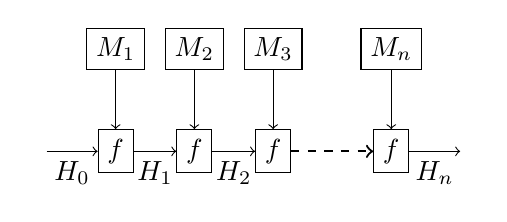
\begin{tikzpicture}[node distance=2cm]
      \node (h_x) at (0,0) {};
      \node (h_y) at (5.5,0) {};
      \begin{scope}[every node/.style={draw}]
        \node (h_0) at (1,0) {\(f\)};
        \node (h_1) at (2,0) {\(f\)};
        \node (h_2) at (3,0) {\(f\)};
        \node (h_n) at (4.5,0) {\(f\)};
      \end{scope}
      \begin{scope}[every node/.style={draw}]
        \node (m_1) at (1,1.3) {\(M_1\)};
        \node (m_2) at (2,1.3) {\(M_2\)};
        \node (m_3) at (3,1.3) {\(M_3\)};
        \node (m_n) at (4.5,1.3) {\(M_n\)};
			\end{scope}
			\begin{scope}[every edge/.style={draw=black,->}]
        \path (h_x) edge node[below] {\(H_0\)} (h_0);
        \path (h_0) edge node[below] {\(H_1\)} (h_1);
        \path (h_1) edge node[below] {\(H_2\)} (h_2);
        \path (h_n) edge node[below] {\(H_n\)} (h_y);

        \path (m_1) edge node[below] {} (h_0);
        \path (m_2) edge node[below] {} (h_1);
        \path (m_3) edge node[below] {} (h_2);
        \path (m_n) edge node[below] {} (h_n);
      \end{scope}
      \begin{scope}[every edge/.style={draw=black,thick,->,dashed}]
				\path (h_2) edge node[below] {} (h_n);
			\end{scope}
    \end{tikzpicture}
  \end{adjustbox}

  %\bibliography{bibliography}
\end{document}
